\documentclass{article}
\usepackage[paperwidth=19cm,paperheight=4.9cm,margin=4mm]{geometry}
\usepackage{amsmath}
\usepackage{tikz}
\usetikzlibrary{arrows.meta,positioning,fit,backgrounds}
\pagestyle{empty}

% Figure Contract
% Core claim: auditable transformations connect observations to verified evidence.
% Evidence: replace every label and value with project model/results artifacts.
% Reader path: left to right.
% Hero: the model-and-constraints stage.
% Supporting evidence: provenance and validation callouts add non-redundant evidence.
% Style: replace with the chosen profile before paper integration.

\begin{document}\noindent
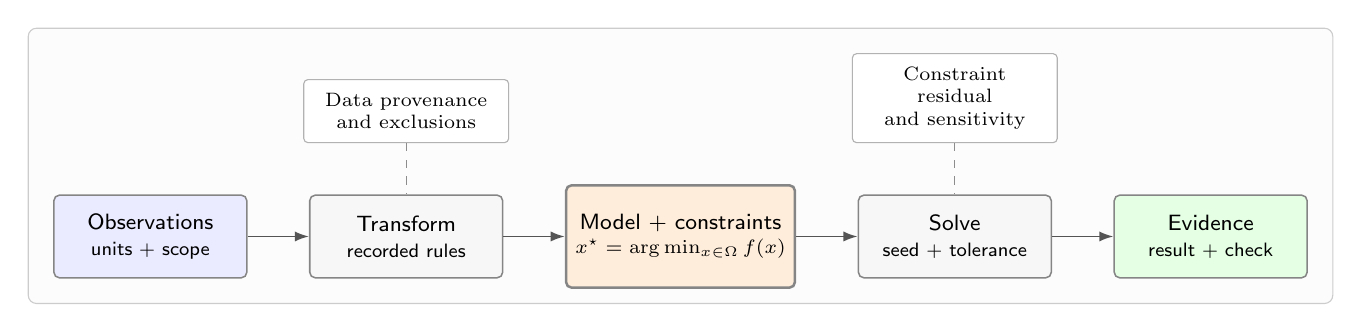
\begin{tikzpicture}[
  font=\sffamily\footnotesize,
  stage/.style={draw=black!48, fill=black!3, rounded corners=2pt,
    minimum width=2.45cm, minimum height=1.05cm, align=center, line width=0.55pt},
  flow/.style={-{Latex[length=1.8mm,width=1.3mm]}, line width=0.7pt, draw=black!67},
  note/.style={draw=black!30, fill=white, rounded corners=1.5pt,
    text width=2.25cm, align=center, font=\scriptsize, inner sep=5pt}
]
  \node[stage, fill=blue!8] (input) {Observations\\\scriptsize units + scope};
  \node[stage, right=0.78cm of input] (transform) {Transform\\\scriptsize recorded rules};
  \node[stage, right=0.78cm of transform, fill=orange!14,
    line width=0.9pt, minimum height=1.30cm] (hero) {Model + constraints\\[-1pt]
      \scriptsize $x^{\star}=\arg\min_{x\in\Omega} f(x)$};
  \node[stage, right=0.78cm of hero] (solve) {Solve\\\scriptsize seed + tolerance};
  \node[stage, right=0.78cm of solve, fill=green!10] (evidence) {Evidence\\\scriptsize result + check};
  \draw[flow] (input) -- (transform);
  \draw[flow] (transform) -- (hero);
  \draw[flow] (hero) -- (solve);
  \draw[flow] (solve) -- (evidence);

  \node[note, above=0.65cm of transform] (provenance) {Data provenance\\and exclusions};
  \draw[black!45, dashed] (provenance) -- (transform);
  \node[note, above=0.65cm of solve] (validation) {Constraint residual\\and sensitivity};
  \draw[black!45, dashed] (validation) -- (solve);

  \begin{scope}[on background layer]
    \node[fit=(input)(evidence)(provenance)(validation), inner sep=9pt,
      fill=black!1, draw=black!20, rounded corners=3pt] {};
  \end{scope}
\end{tikzpicture}
\end{document}
